\chapter{\texorpdfstring{WF-nets Construction}{WF-nets Construction}}
\label{ch:13}
\lecturemeta{Lezione 13 \quad\textbullet\quad 2026-07-03 \quad\textbullet\quad Roberto Bruni}{Petri nets · workflow nets}

In \hyperref[ch:12]{12 — Soundness} abbiamo definito la soundness e imparato a \textbf{verificarla} su una rete data (via il teorema $N$ sound $\iff N^\star$ live+bounded). Ma la verifica ha un limite: se la rete risulta \emph{non} sound, non ci dice come ripararla, e su reti grandi costa (state explosion). Questa lezione ribalta il problema: invece di \textbf{verificare} la soundness a posteriori, la \textbf{garantisce per costruzione}. Si parte da mattoni elementari già dimostrati corretti e li si compone con regole che \textbf{preservano} la correttezza — così il risultato è sound e safe \emph{by design}, senza bisogno di analizzarlo.

\section{\texorpdfstring{L'idea: costruire, non verificare}{L'idea: costruire, non verificare}}

La strategia ha due ingredienti.

\begin{boxtip}{Soundness per costruzione}
\begin{enumerate}
\item Trovare un insieme di \textbf{building block}: piccoli workflow net di cui è \textbf{facile dimostrare} che sono \textbf{sound} e \textbf{safe} (1-bounded).
\item Definire dei \textbf{pattern di composizione} tali che, \textbf{componendo} WF net safe e sound, si ottiene ancora un WF net safe e sound.
\end{enumerate}
\end{boxtip}

Il cuore della tecnica è un'operazione di \textbf{sostituzione} (refinement): prendere una transizione di una rete e "esploderla", rimpiazzandola con un intero workflow net.

\begin{boxdefinition}{Composizione $N[N'/t]$}
Siano $N$ e $N'$ due workflow net safe e sound. Sia $t$ una \textbf{task di $N$ con esattamente un input place e un output place}. La rete $N[N'/t]$ si ottiene \textbf{rimpiazzando la task $t$ in $N$ con l'intera rete $N'$} (collegando i punti d'ingresso/uscita di $N'$ al posto di $t$).
\end{boxdefinition}

\begin{boxtheorem}{Il teorema di composizione}
Se $N$ e $N'$ sono workflow net safe e sound, allora $N[N'/t]$ è un workflow net \textbf{safe e sound} (dimostrazione omessa).
\end{boxtheorem}

\begin{boxabstract}{Perché funziona (intuizione)}
Un workflow net sound, visto \textbf{da fuori}, si comporta \emph{esattamente come una transizione}: prende un token dal suo input place e ne produce uno nel suo output place — solo, \textbf{non atomicamente} (nel mezzo fa il suo lavoro interno). Quindi rimpiazzare una transizione con un WF net sound non altera il comportamento globale. Formalmente, la dimostrazione costruisce una \textbf{corrispondenza biunivoca} tra le marcature della rete composta $N[N'/t]$ e le \textbf{coppie} di marcature di $N$ e $N'$.
\end{boxabstract}

Perché il collegamento funzioni, servono due lemmi sulle transizioni "di bordo":

\begin{boxnote}{Transizioni iniziali e finali}
\begin{itemize}
\item Una transizione $t$ è \textbf{iniziale} se c'è un arco dal place iniziale $i$ a $t$. In un WF net sound, se $t$ è iniziale allora:
\end{itemize}

\[
\bullet t = \{i\}
\]

(altrimenti $t$ sarebbe dead, perché all'inizio l'unico token è in $i$). - Una transizione $t$ è \textbf{finale} se c'è un arco da $t$ al place finale $o$. In un WF net sound, se $t$ è finale allora:

\[
t\bullet = \{o\}
\]

(altrimenti $t$ sarebbe dead, oppure violerebbe la proper completion lasciando token oltre a quello in $o$).

Questi vincoli assicurano che, sostituendo $N'$ al posto di $t$, le sue transizioni iniziali si aggancino puliti all'input di $t$ e quelle finali all'output.
\end{boxnote}

\section{\texorpdfstring{Il catalogo dei building block}{Il catalogo dei building block}}

Ecco i mattoni di base, tutti workflow net sound e safe (verificabili a mano). Sono le "istruzioni" con cui comporre qualunque processo.

\begin{figure}[!htb]
\centering
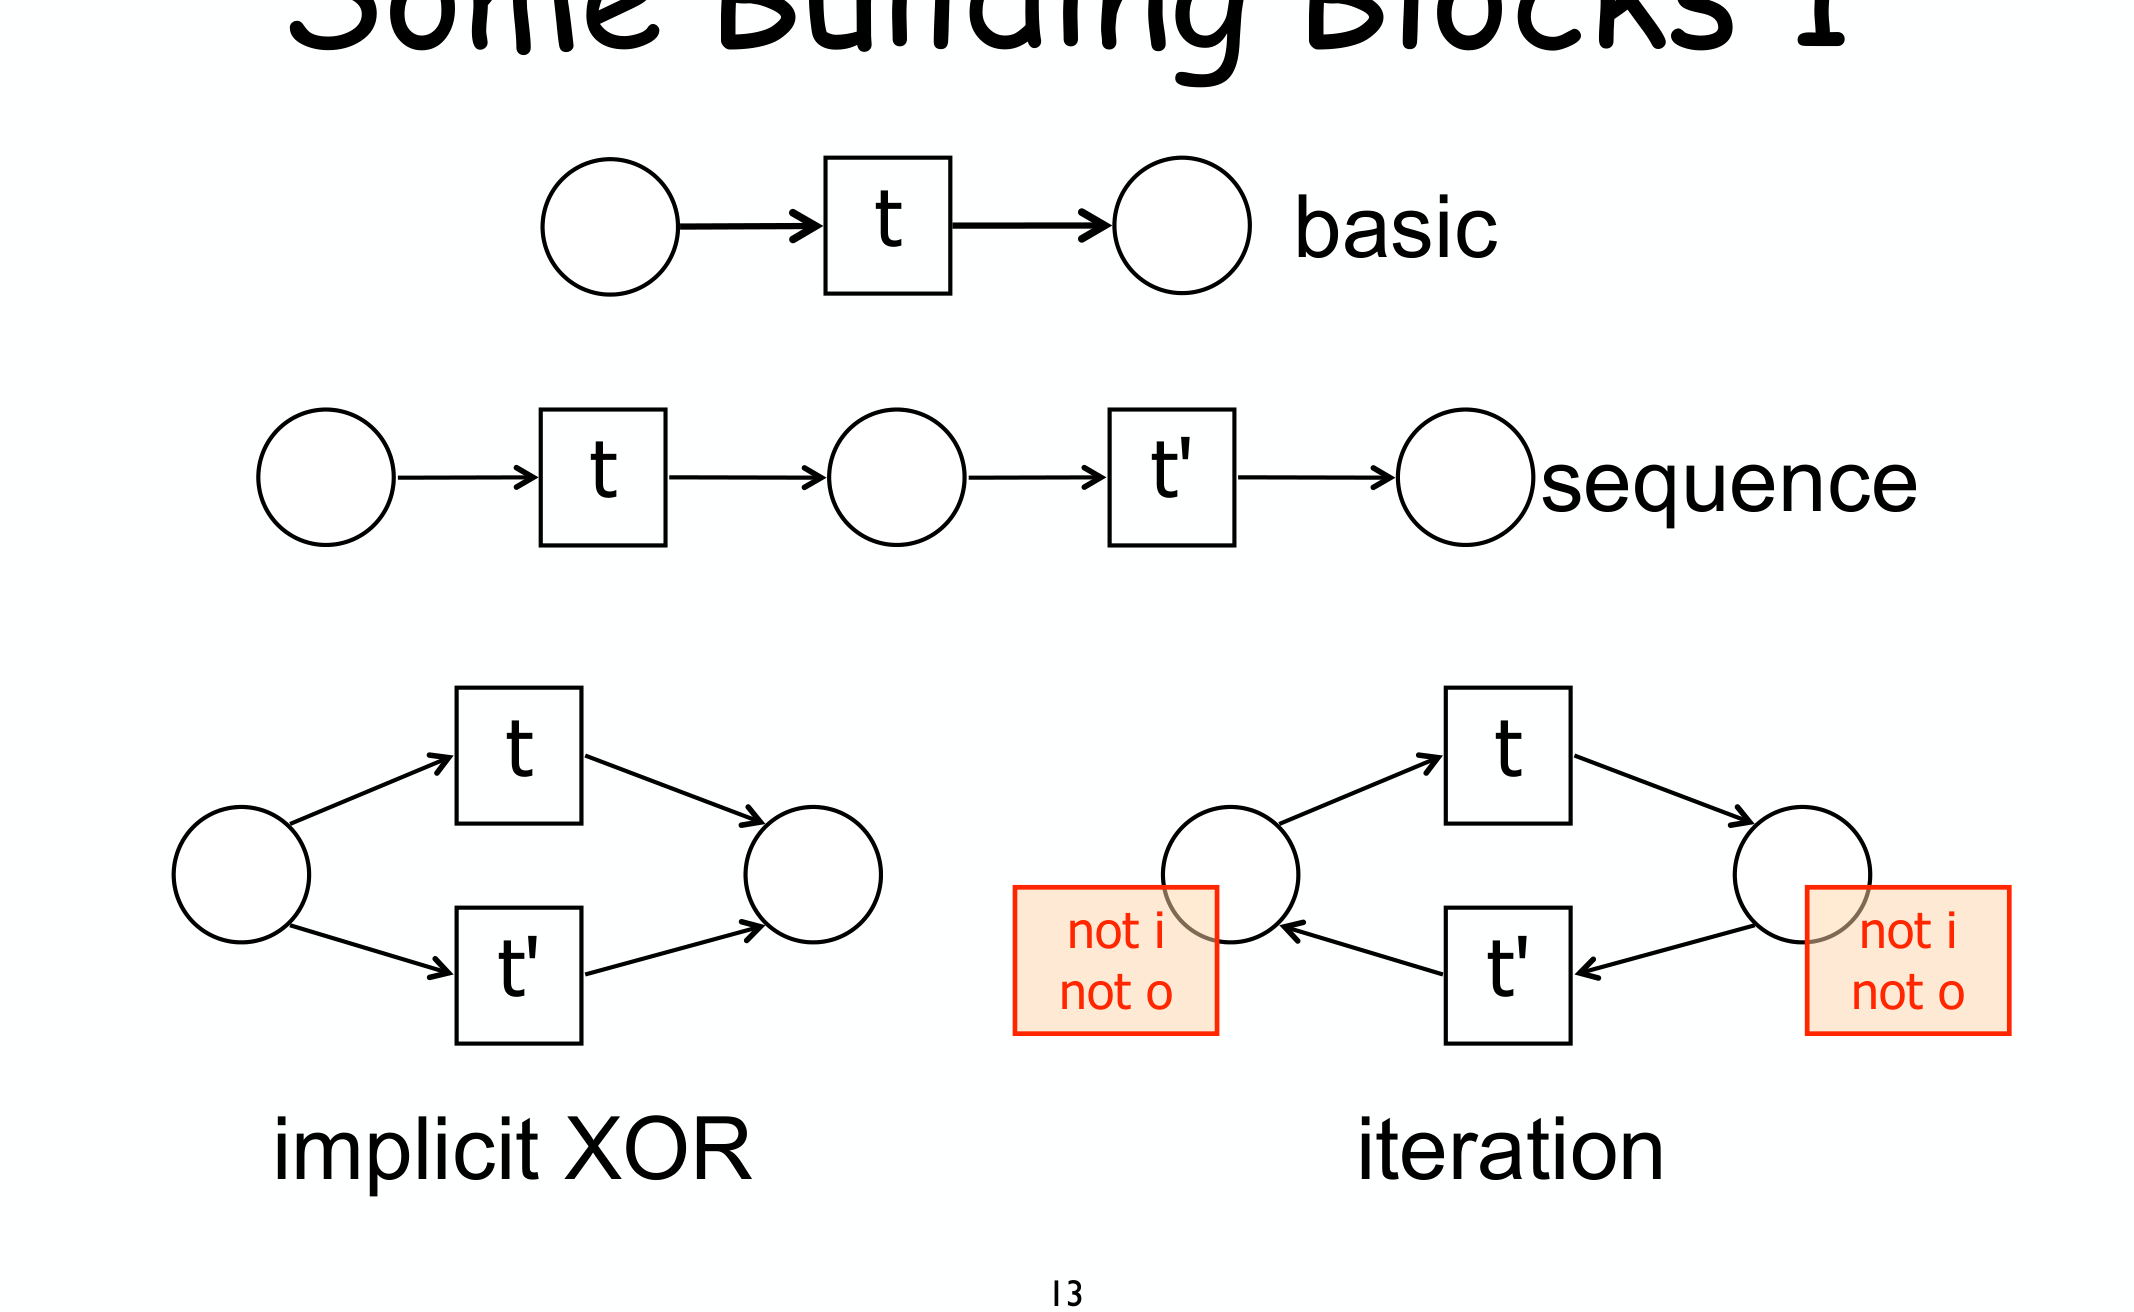
\includegraphics[width=0.74\linewidth,height=0.34\textheight,keepaspectratio]{images/13-wfnets_p12_building-blocks.png}
\caption{Building blocks 1. \textbf{Basic}: la singola task. \textbf{Sequence}: $t$ poi $t'$. \textbf{Implicit XOR}: dal place iniziale, $t$ \emph{oppure} $t'$ (scelta implicita, deferred). \textbf{Iteration}: un ciclo che può ripetersi; i place laterali sono marcati "not i / not o" perché un blocco interno non può usare direttamente l'ingresso/uscita globali.}
\end{figure}

Oltre a questi ci sono le varianti esplicite della scelta e la concorrenza:

\begin{itemize}
\item \textbf{Explicit XOR-split / XOR-join}: la scelta risolta da una transizione dedicata (invece che dalla competizione sul place).
\item \textbf{XOR block}: split e join esplicito racchiusi in un blocco.
\item \textbf{AND (parallel)}: la concorrenza vera dei Petri net, con una transizione che apre due rami e una che li richiude.
\end{itemize}

\begin{figure}[!htb]
\centering
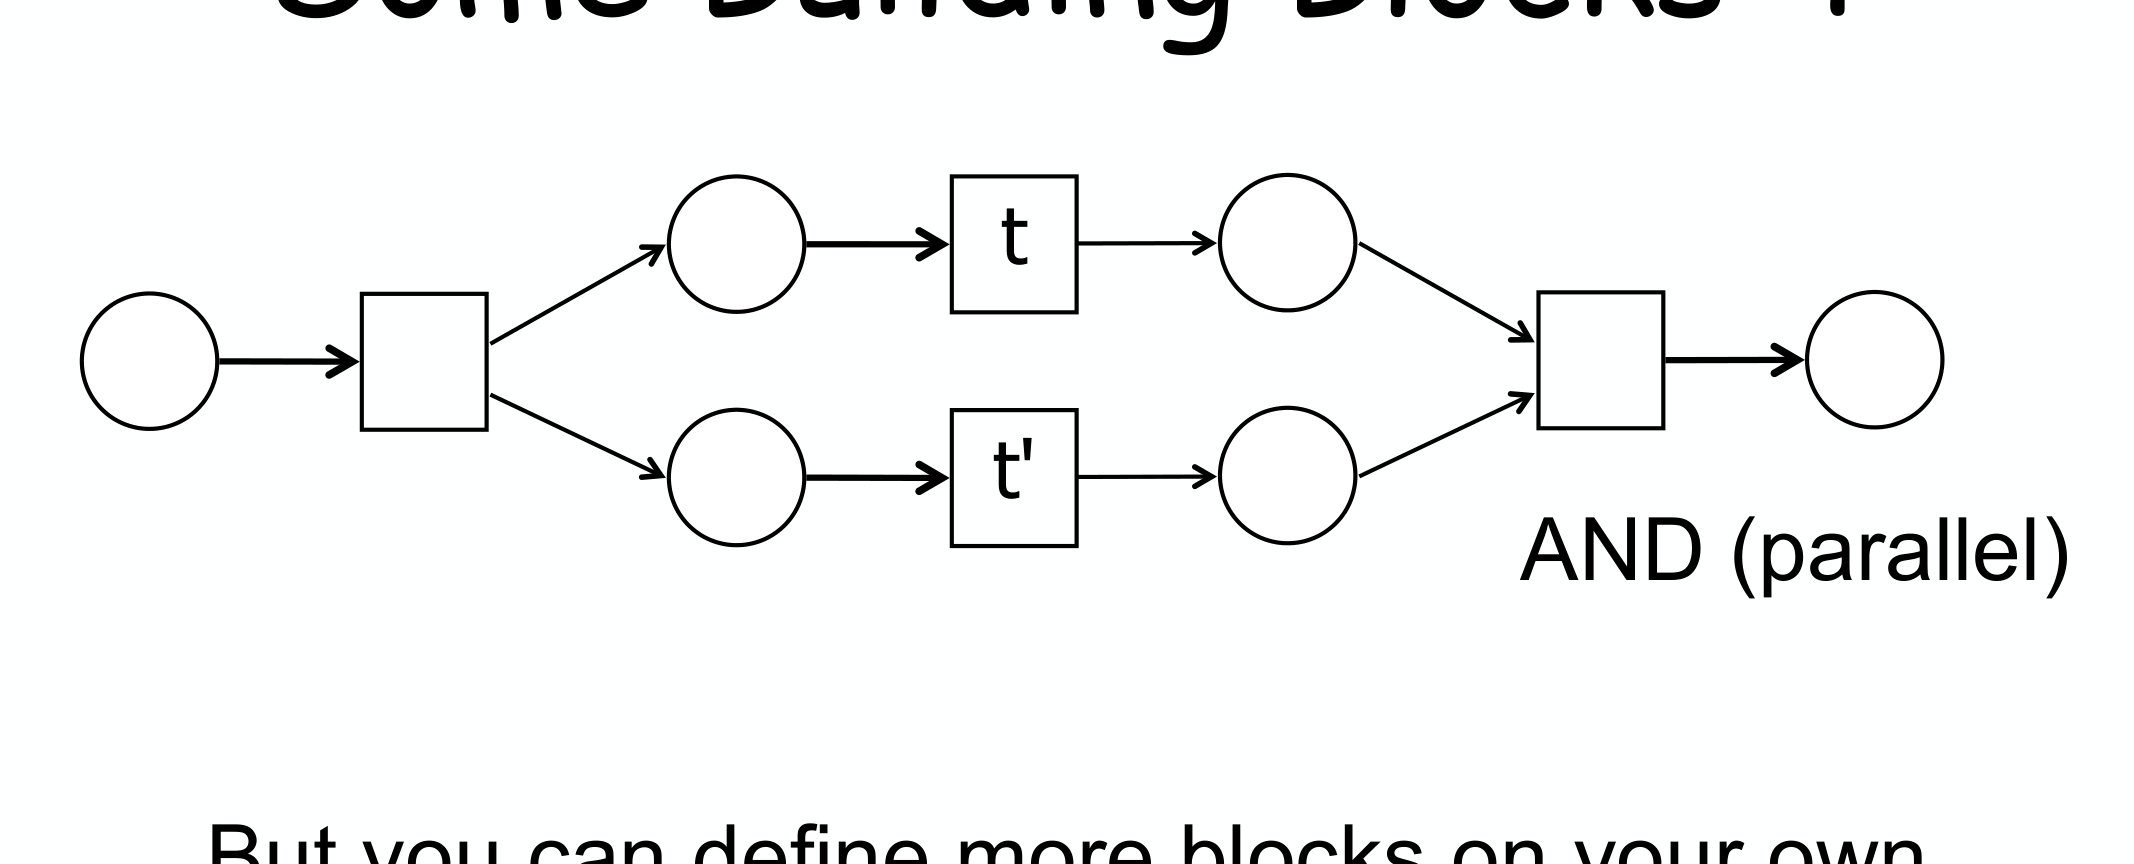
\includegraphics[width=0.74\linewidth,height=0.34\textheight,keepaspectratio]{images/13-wfnets_p15_and-block.png}
\caption{Il blocco \textbf{AND (parallel)}: una transizione di split attiva entrambi i rami $t$ e $t'$, una di join attende il completamento di entrambi. È il pattern di parallelismo dei Petri net (\hyperref[ch:04]{04 — Petri Nets}). Esiste anche una variante \textbf{AND with sync}. E, naturalmente, "you can define more blocks on your own".}
\end{figure}

\section{\texorpdfstring{Refinement e abstraction}{Refinement e abstraction}}

La composizione si usa in due direzioni complementari:

\begin{itemize}
\item \textbf{Refinement} (raffinamento): si parte da una rete astratta e si \textbf{espande} progressivamente una transizione alla volta, sostituendola con un blocco più dettagliato. Ogni passo preserva soundness e safeness.
\item \textbf{Abstraction} (astrazione): il procedimento inverso, utile per \textbf{dimostrare} che una rete complessa è sound — la si "riconosce" come composizione di blocchi noti, riducendola passo dopo passo (una iteration qui, un XOR block lì, una sequence, un blocco parallelo...) fino a un unico blocco basic. Se ogni riduzione è un pattern valido, la rete di partenza è sound per costruzione.
\end{itemize}

\subsection{\texorpdfstring{Esempio di design: Car Damage}{Esempio di design: Car Damage}}

L'esempio riassuntivo è un processo assicurativo di gestione danni auto, costruito interamente componendo blocchi:

\begin{figure}[!htb]
\centering
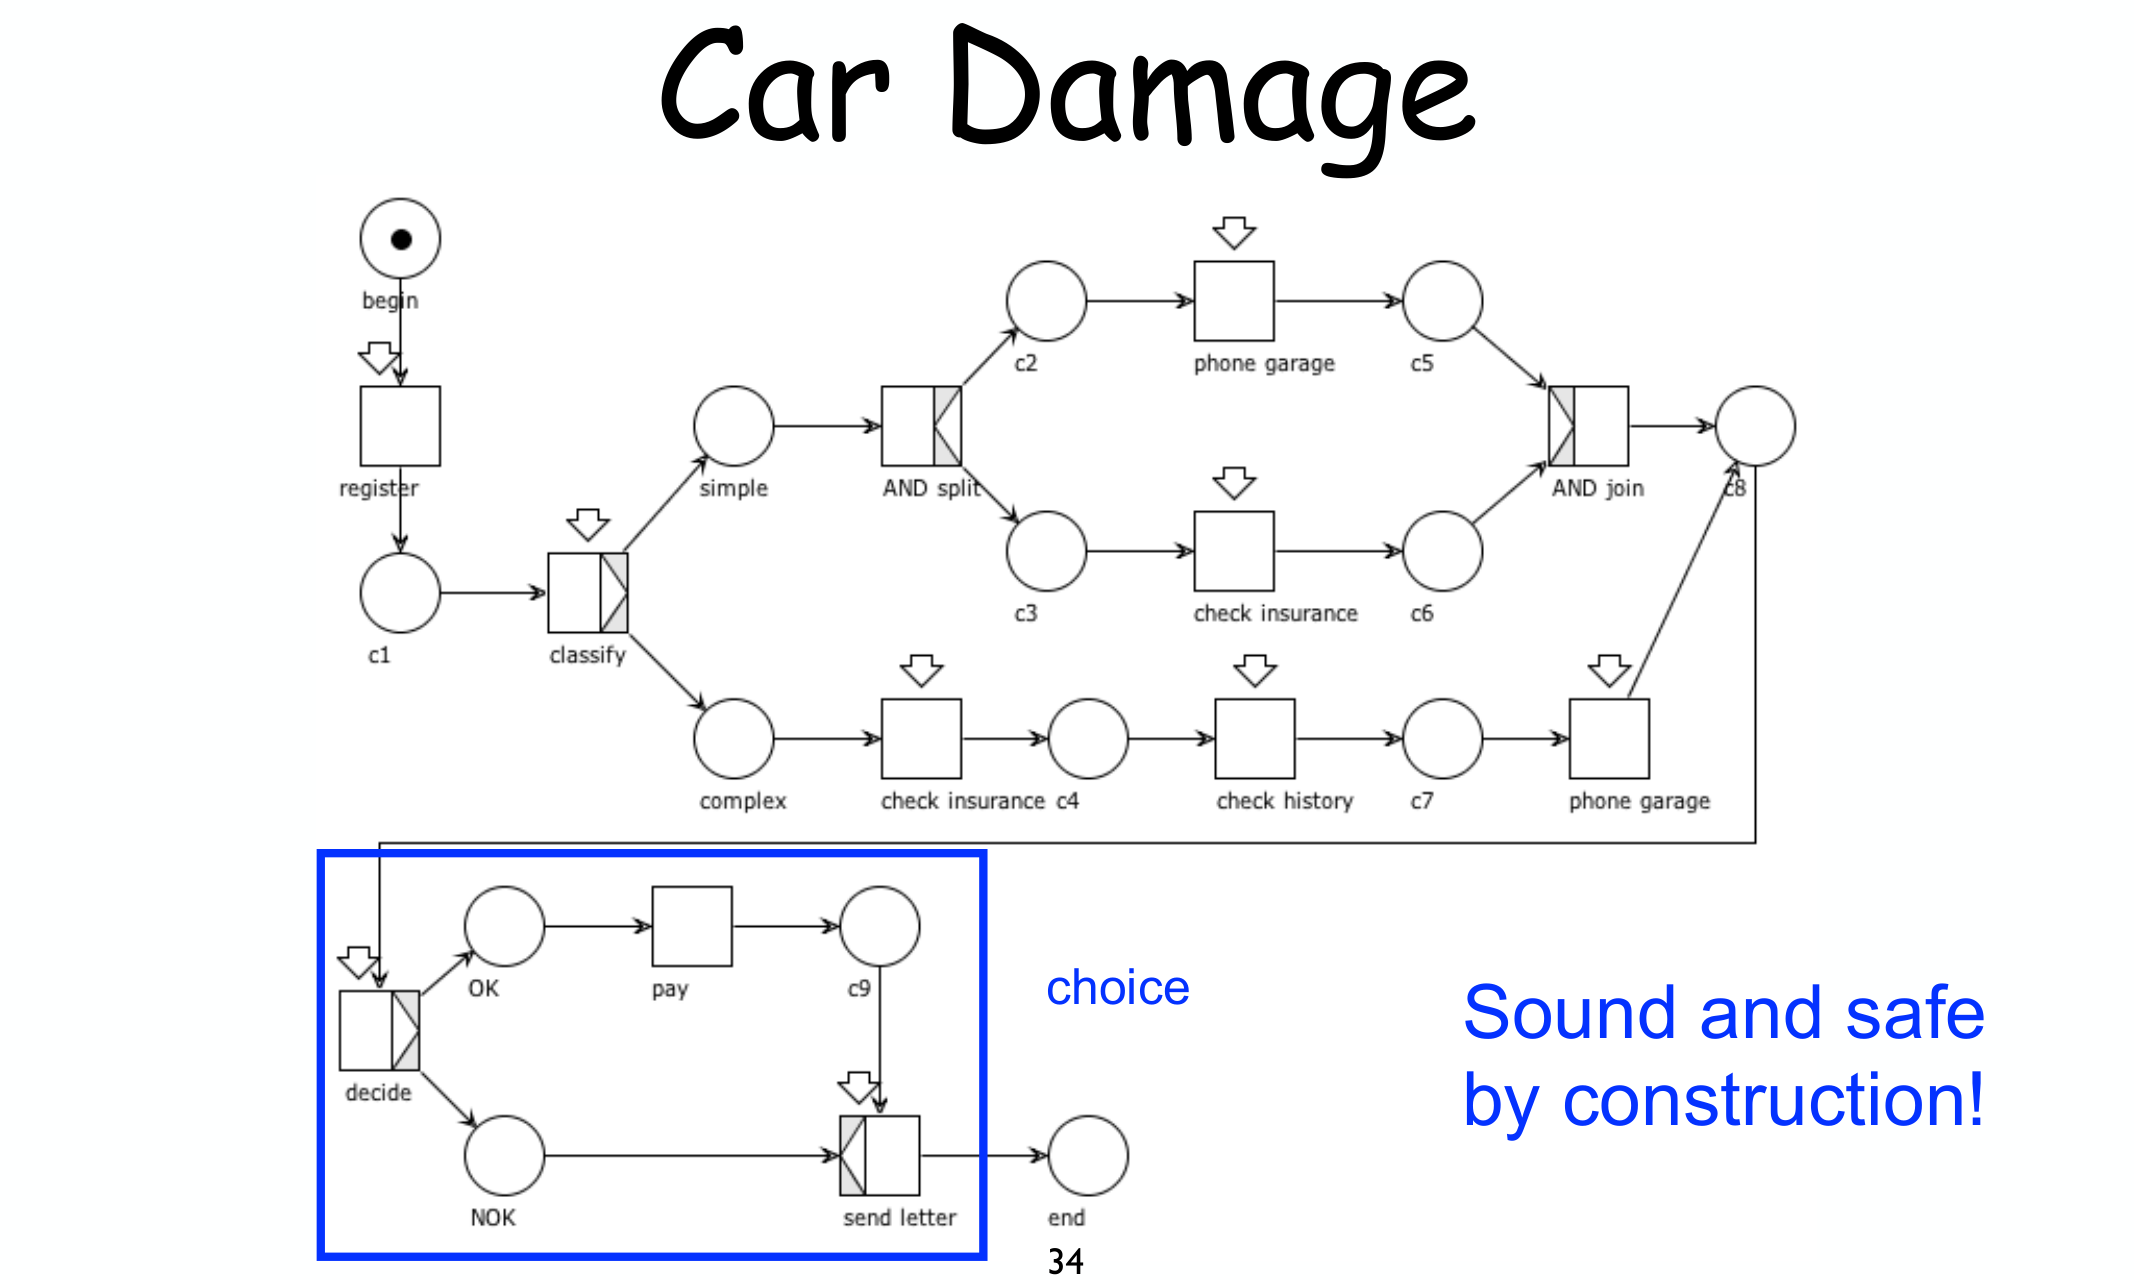
\includegraphics[width=0.74\linewidth,height=0.34\textheight,keepaspectratio]{images/13-wfnets_p33_car-damage.png}
\caption{Design del Car Damage. Il processo è assemblato da blocchi: \textbf{choice} (classify: simple/complex; decide: OK/NOK), \textbf{AND parallel} (phone garage $\parallel$ check insurance nel ramo simple), \textbf{sequence} (nel ramo complex). Essendo ogni blocco sound+safe e le composizioni valide, il risultato è \textbf{"sound and safe by construction"} — senza costruire il reachability graph.}
\end{figure}

\section{\texorpdfstring{Generalizzazione: sostituire transizioni con più archi}{Generalizzazione: sostituire transizioni con più archi}}

Finora abbiamo raffinato solo task con \textbf{un} input e \textbf{un} output. Il metodo si estende a transizioni con \textbf{più archi entranti e uscenti}, con una regola di ricablaggio precisa.

\begin{figure}[!htb]
\centering
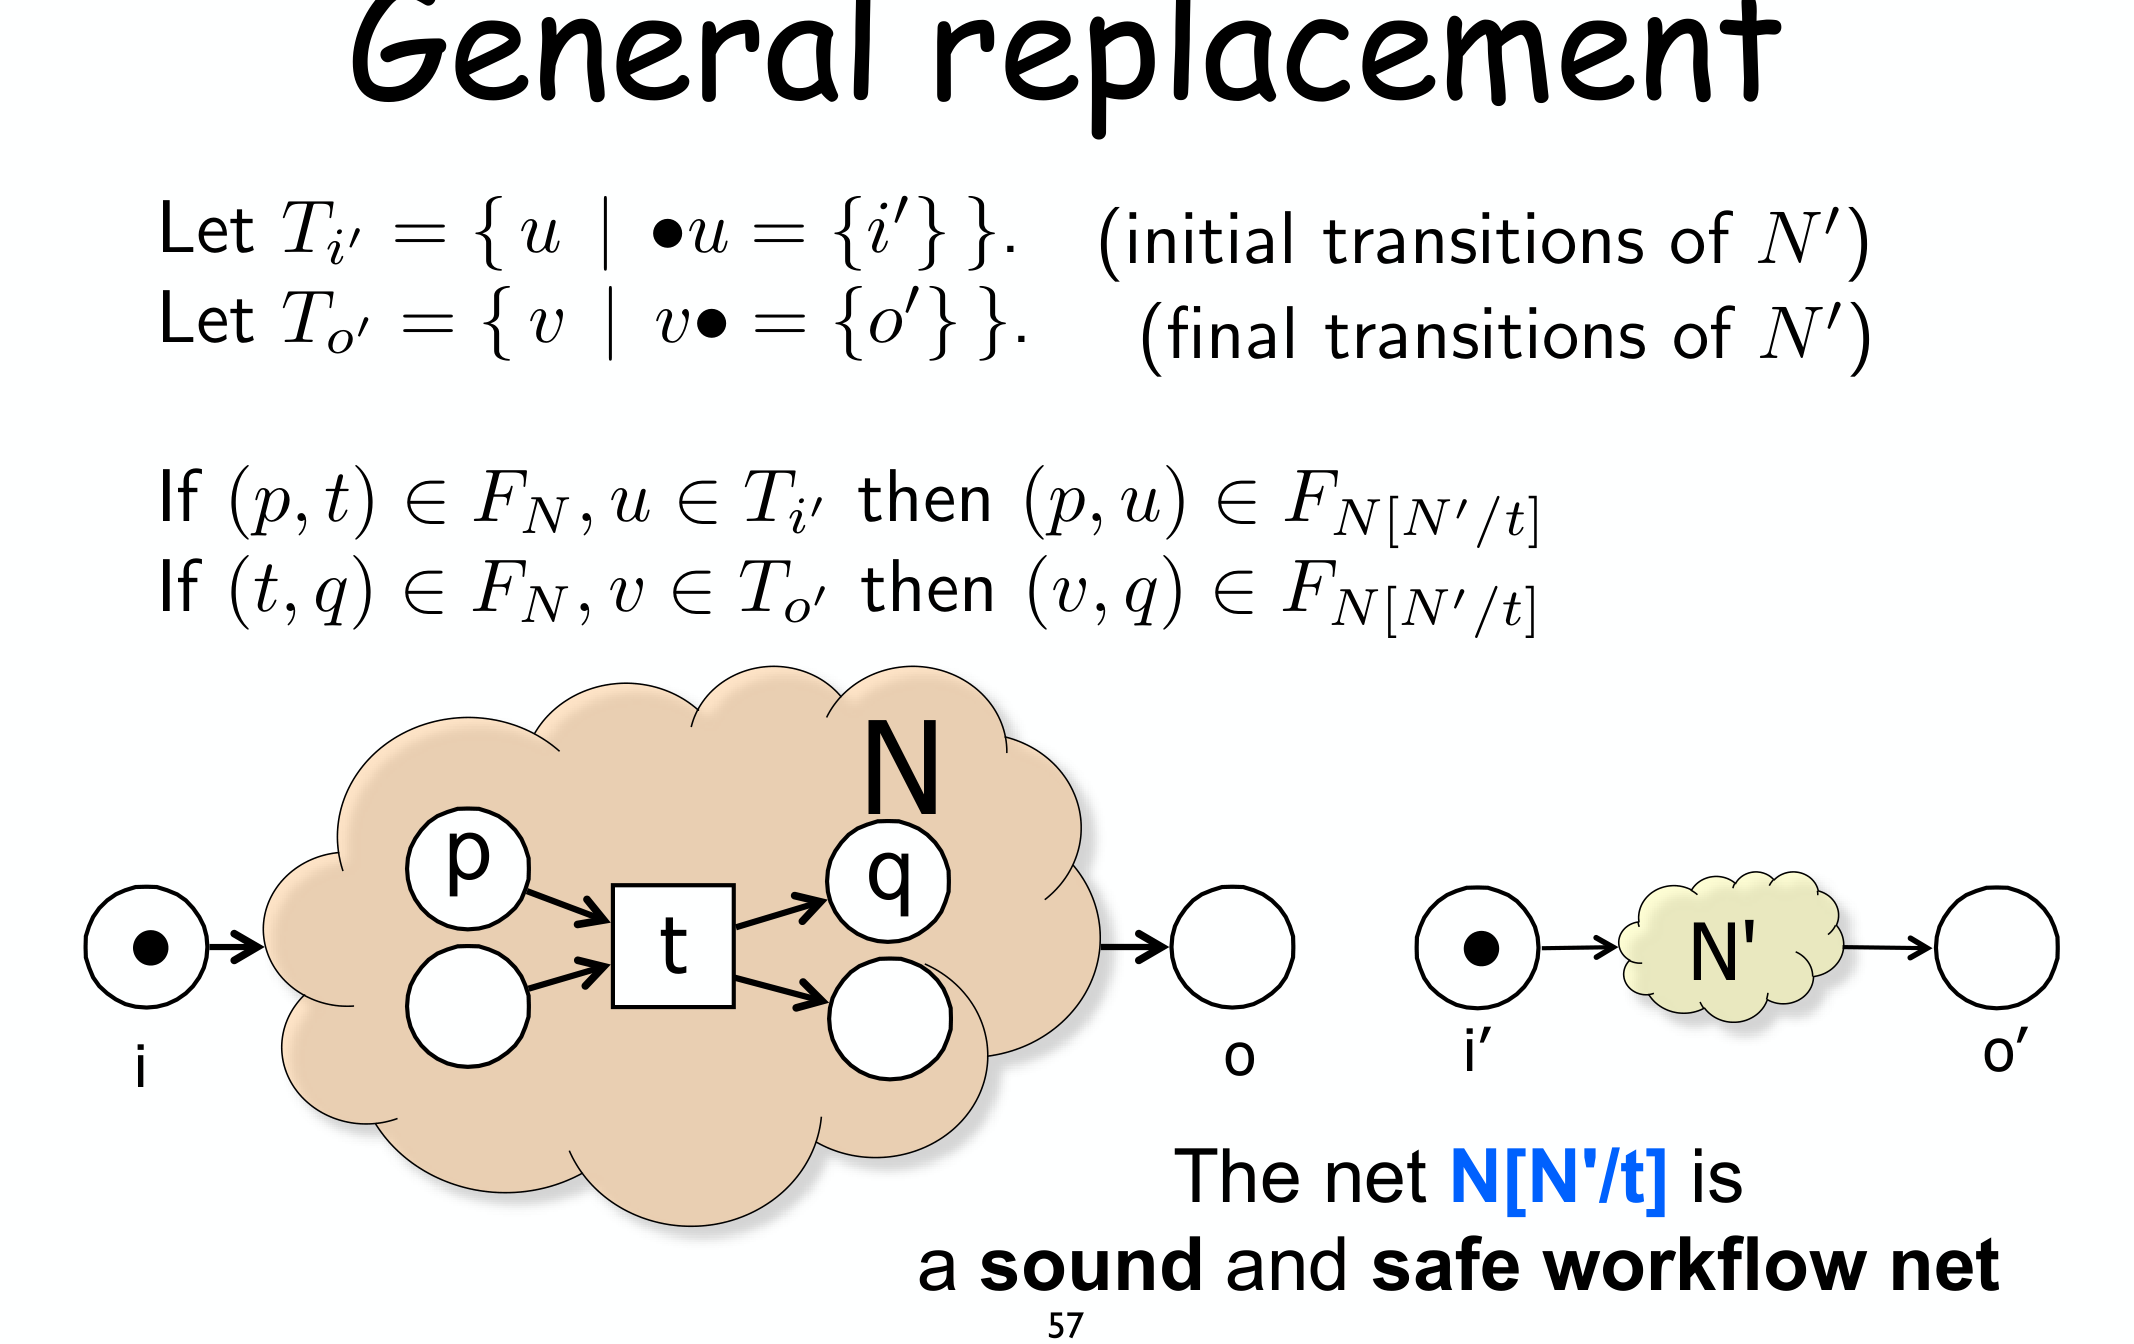
\includegraphics[width=0.74\linewidth,height=0.34\textheight,keepaspectratio]{images/13-wfnets_p56_general-replacement.png}
\caption{General replacement. Detti $T_{i'} = \{u \mid \bullet u = \{i'\}\}$ le transizioni \textbf{iniziali} di $N'$ e $T_{o'} = \{v \mid v\bullet = \{o'\}\}$ le \textbf{finali}, il ricablaggio è: ogni arco $(p,t)$ di $N$ diventa $(p, u)$ per ogni transizione iniziale $u$; ogni arco $(t,q)$ diventa $(v, q)$ per ogni transizione finale $v$. Anche così, $N[N'/t]$ resta un WF net \textbf{sound e safe}.}
\end{figure}

\begin{boxtip}{Il valore pratico della tecnica}
Costruire per composizione dà \textbf{due garanzie gratis}: la rete è sound (nessun deadlock, nessun token pendente, nessuna task morta) e safe (1-bounded), \textbf{senza analisi}. È l'analogo, per i processi, della programmazione strutturata: comporre costrutti corretti (sequenza, scelta, ciclo, parallelo) dà programmi corretti per costruzione. Il prezzo è una minor libertà — non tutti i WF net sound sono ottenibili così — ma per il design pratico è un ottimo compromesso.
\end{boxtip}

Con la costruzione per blocchi chiudiamo la teoria fondamentale dei workflow net. Le prossime lezioni introdurranno strumenti di analisi più avanzati, come gli \textbf{invarianti}. $\rightarrow$ \hyperref[ch:14]{14 — Invariants}